\documentclass[serif,mathserif]{beamer}
\geometry{paperwidth=150mm,paperheight=105mm}
\setbeamersize{text margin left=1.4cm,text margin right=1.4cm} 
\usepackage{amsmath, amsfonts, epsfig, xspace}
\usepackage{adjustbox}
\usepackage{algorithm,algorithmic}
\usepackage{pstricks,pst-node}
\usepackage[normal,tight,center]{subfigure}
\setlength{\subfigcapskip}{-.5em}
\usepackage{beamerthemesplit}
\usetheme{lankton-keynote}
\usepackage{units}
\usepackage{graphicx}

\graphicspath{{./figures/}}

\author[Kevin Liu Rodrigues]{Kevin Liu Rodrigues}
\title[frame \hspace{2em}\insertframenumber/\inserttotalframenumber]{Synchronization on Discrete Oscillators}
\institute{Federal University of Minas Gerais}

\begin{document}

\maketitle

\begin{frame}{Motivations}
    Belousov-Zhabotinsky reaction (1960)
    \begin{itemize}
        \item \ \pause Establishment of non-linear chemical oscillators
        \item \ \pause Evolves chaotically for long periods of time
        \item \ \pause Chemical reactions not necessarily dominated by equilibrium thermodynamics
    \end{itemize}
\end{frame}

\begin{frame}{Motivations}
    \begin{columns}[t]
        \begin{column}{.6\textwidth}
            \adjincludegraphics[width=0.7\textwidth, valign=t]{bz.eps}
        \end{column}
        \begin{column}{.4\textwidth}
            Simulation of the B-Z reaction on a 2-D Petri dish.
        \end{column}
    \end{columns}
\end{frame}

\begin{frame}{Motivations}
    \begin{columns}[t]
        \begin{column}{0.6\textwidth}
            \adjincludegraphics[width=.9\linewidth, valign=t]{bbc.eps}
        \end{column}
        \begin{column}{0.4\textwidth}
            BBC United Kingdom (2010) ``Wet computing''
            \begin{itemize}
                \item \ \pause B-Z reactions inside lipid layers
                \item \ \pause Refractory period similar to neurons
            \end{itemize}
        \end{column}
    \end{columns}
\end{frame}

\begin{frame}{The Model}
    Oscillators are characterized by a discrete phase value which jumps \textbf{\textit{stochastically}} from one phase to the next.
    \begin{itemize}
        \vspace{0.25cm}
        \item \ \pause 3 discrete phase values for each state $x_i$: \\
        $\qquad \phi_{x_i} = x_i\frac{2\pi}{3}, \quad x_i \in \{0,1,2\}$
        \vspace{0.25cm}
        \item \ \pause States cycle in one direction: $0 \rightarrow 1 \rightarrow 2 \rightarrow 0 \rightarrow \dots$ \\
            $\qquad x_i(t+1) = x_i(t) + 1 \mod 3$
        \vspace{0.25cm}
        \item \ \pause \textbf{\textit{Isolated}} oscillators transition with intrinsic rate $g$
        \vspace{0.25cm}
        \item \ \pause \textbf{\textit{Coupled}} oscillators have altered transition rates depending on its internal state and those of its neighbors
    \end{itemize}
\end{frame}

\begin{frame}{The Model}
    \begin{columns}[t]
        \begin{column}{0.5\textwidth}
            \centering
            \adjincludegraphics[width=0.9\linewidth, valign=t]{wood-model.eps}
        \end{column}
        \begin{column}{0.6\textwidth}
            Coupling function $\Gamma_i = \exp \left( a \frac{K_i^{x_i + 1} - K_i^{x_i}}{K_i} \right)$ \\
            $K_{i}$: Number of neighbors of oscillator $i$
            $K_i^{x_i}$: Among $K_i$, this is the number of neighbors in state $x_i$ \\
            \begin{itemize}
                \vspace{0.25cm}
                \item \ \pause Free oscillators have transition rate $g$
                \vspace{0.25cm}
                \item \ \pause Coupled oscillators influence each others transitions rates according to the coupling function $\Gamma$
                \vspace{0.25cm}
                \item \ \pause The strength of the coupling is modulated by $a$
            \end{itemize}
        \end{column}
    \end{columns}
\end{frame}

\begin{frame}{The model}
    \begin{columns}
        \begin{column}{0.4\textwidth}
            \adjincludegraphics[width=0.9\linewidth, valign=t]{order-parameter.eps}
        \end{column}
        \begin{column}{0.6\textwidth}
            Oscillators as vectors in the unit circle
            \begin{itemize}
                \vspace{0.25cm}
                \item \ \pause Synchronicity can be measured by summing the phases
                \vspace{0.25cm}
                \item \ \pause $\left< \right>_t$: \textit{\textbf{time}} average\\
                    \hspace{0.1cm}$\left< \right>_s$: average over \textit{\textbf{independent trials}}
                \vspace{0.25cm}
                \item \ \pause $\chi_r$ is the scaled variance of the order parameter $r$
                \vspace{0.25cm}
                \item \ \pause $\psi$: order parameter (infinite period transition)
            \end{itemize}
        \end{column}
    \end{columns}
\end{frame}

\begin{frame}
    All-to-all graphs
    \begin{itemize}
        \vspace{0.35cm}
        \item \ \pause $\frac{N^x}{N} \rightarrow P(x)$: probability of finding a given vertex in state $x$
        \vspace{0.35cm}
        \item \ \pause Only three possible transition rates: $\Gamma^x = \exp \left[ a (P(x+1) - P(x)) \right]$
        \vspace{0.35cm}
        \item \ \pause Master equations: $\dot P(x) = \Gamma^{x-1}P(x-1) - \Gamma(x)P(x), \quad x \in \{0, 1, 2\}$
        \vspace{0.35cm}
        \item \ \pause Order parameter simplified:\\
        \begin{equation*}
            \begin{split}
                |\psi| = \frac{1}{N} [
                & \left(N^0\Gamma^0\right)^2
                + \left(N^1\Gamma^1\right)^2
                + \left(N^2\Gamma^2\right)^2\\
                & - N^0N^1\Gamma^0\Gamma^1
                - N^0N^2\Gamma^0\Gamma^2
                - N^1N^2\Gamma^1\Gamma^2
            ]^{1/2}
            \end{split}
        \end{equation*}
        \vspace{0.35cm}
        \item \ \pause Fixed point $P(0) = P(1) = P(2) = \frac{1}{3}$ becomes unstable when $a>1.5$
    \end{itemize}
\end{frame}

\begin{frame}
    \centering
    Behavior of $\psi$ as a function of coupling for the all-to-all graph\\
    \vspace{0.8cm}
    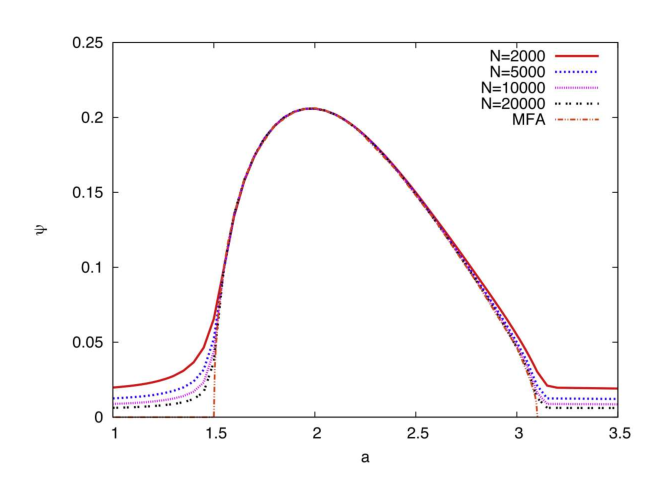
\includegraphics[height=0.7\textheight]{psi-vs-a.eps}\\
    Vladimir R V Assis et al J. Stat. Mech. (2011) P09023
\end{frame}

\begin{frame}
    \centering
    Evolution of population of states as a function of time\\
    \vspace{0.8cm}
    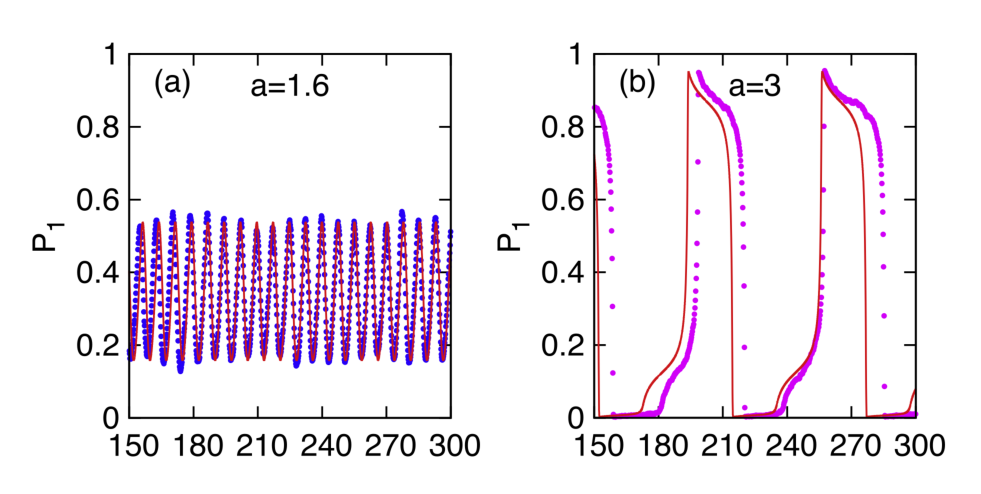
\includegraphics[height=0.6\textheight]{pop-evolution.eps}\\
    Vladimir R V Assis et al J. Stat. Mech. (2011) P09023
\end{frame}

\begin{frame}
    \centering
    Frequency of oscillations and order parameter $r$ as functions of coupling\\
    \vspace{0.8cm}
    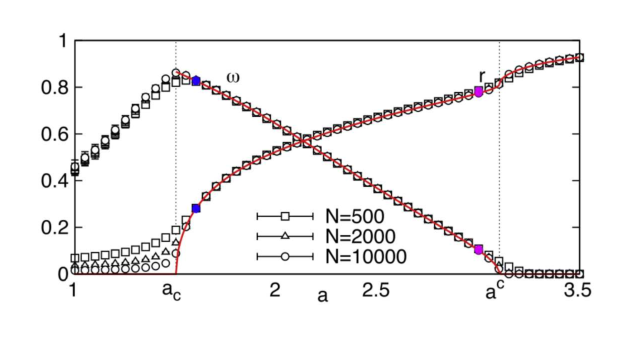
\includegraphics[height=0.6\textheight]{rvsa.eps}\\
    Vladimir R V Assis et al J. Stat. Mech. (2011) P09023
\end{frame}

\begin{frame}
    \centering
    Event driven dynamics simulation on the complete graph\\
    \vspace{0.8cm}
    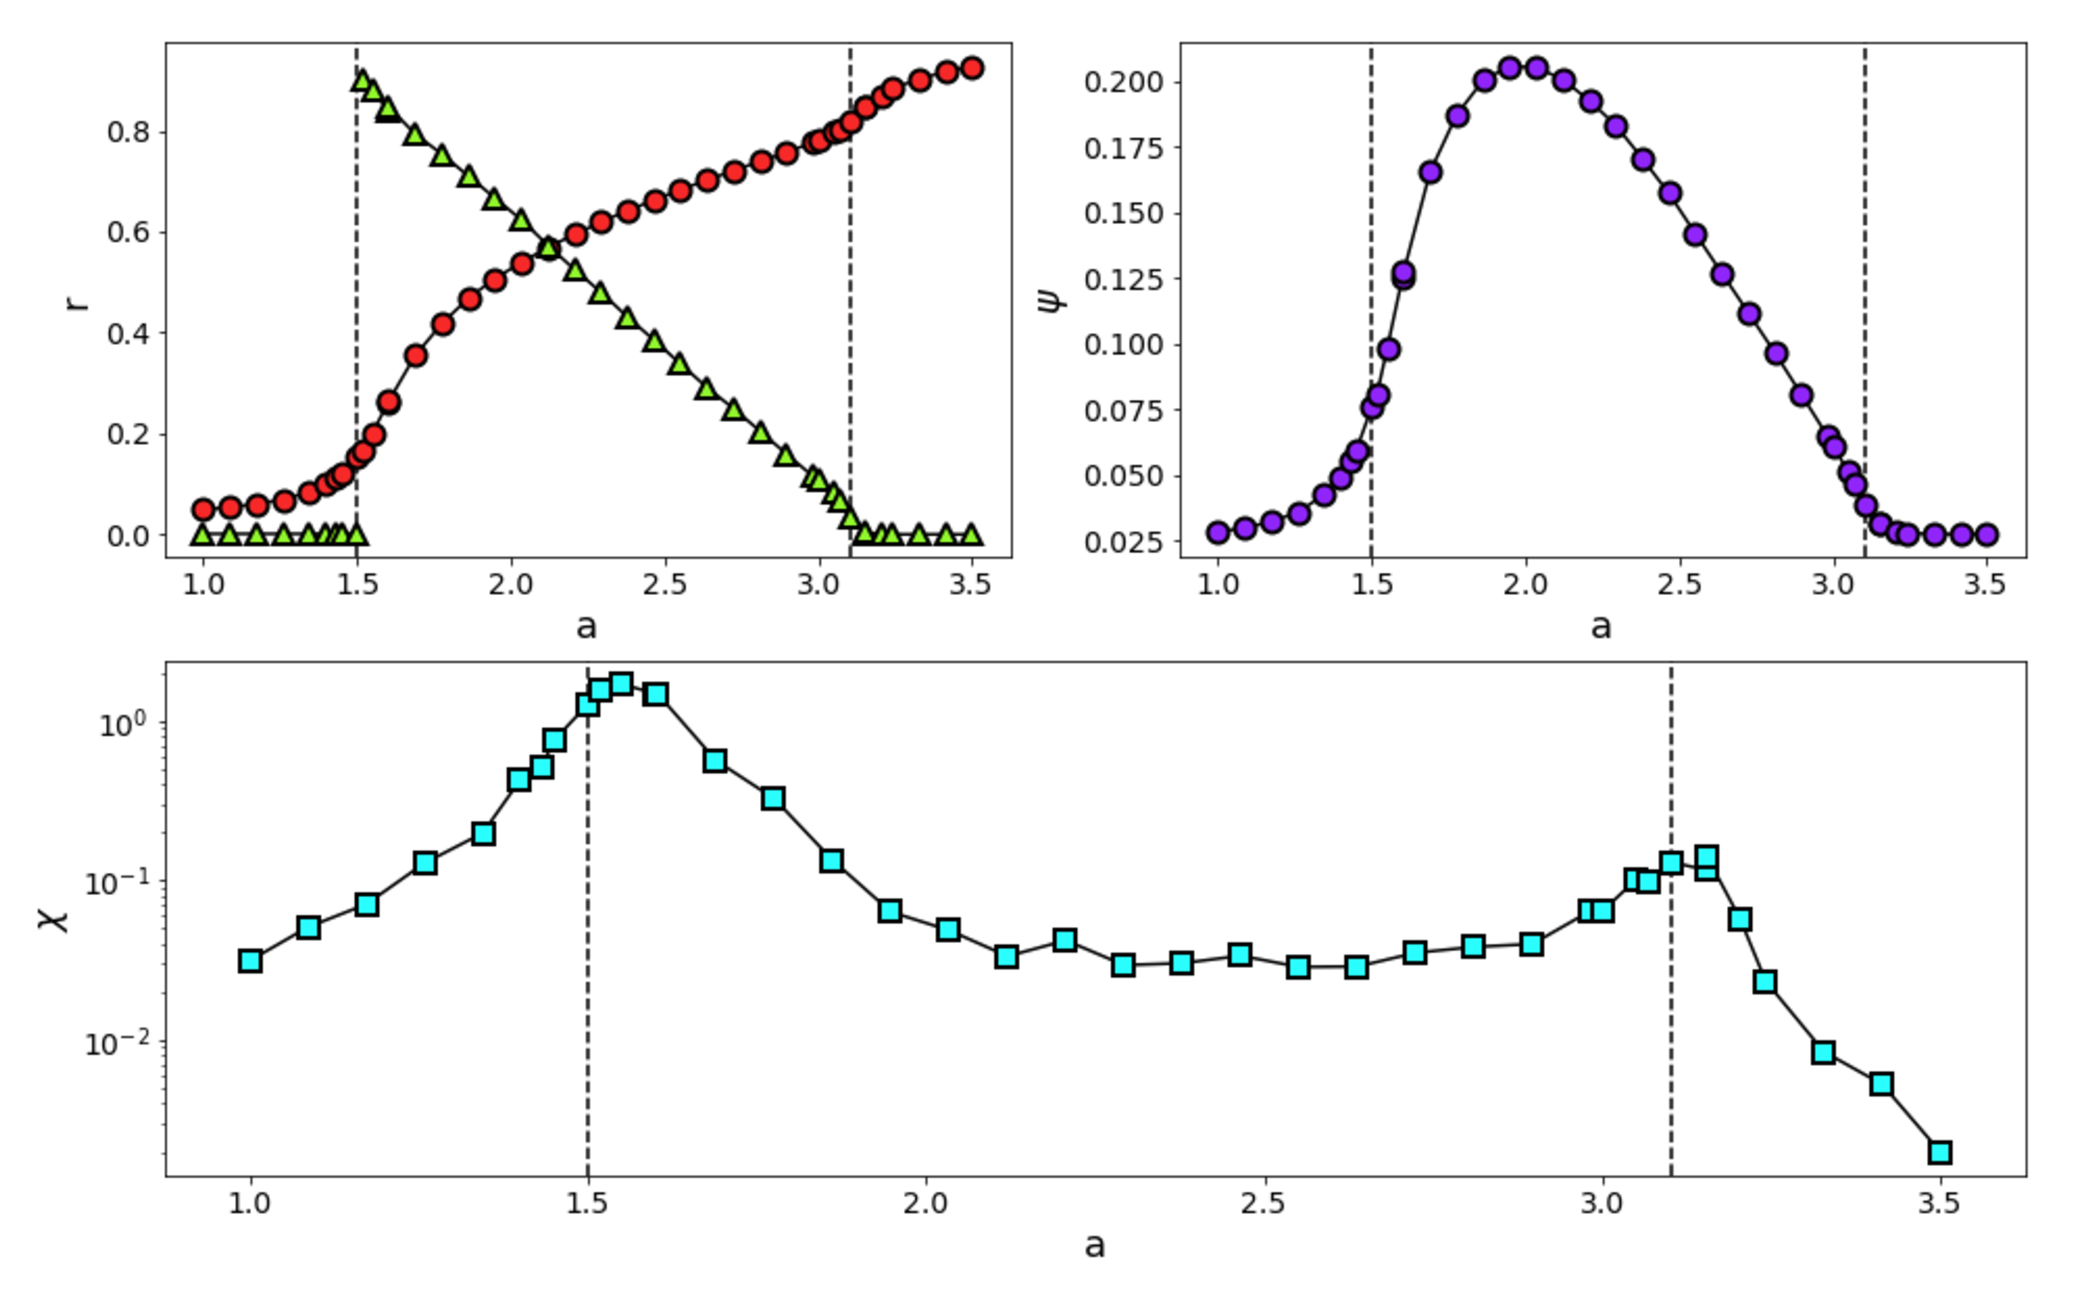
\includegraphics[width=\textwidth]{complete_graph.eps}
\end{frame}

\begin{frame}
    The all-to-all coupling presents two phase transitions
    \begin{itemize}
        \vspace{0.35cm}
        \item \ \pause At $a=a_c=1.5$ there is the onset of global oscillations
        \vspace{0.35cm}
        \item \ \pause At $a=a^c\approx 3.1$ the period of oscillations diverge as $\omega=0$
    \end{itemize}
\end{frame}

\begin{frame}
    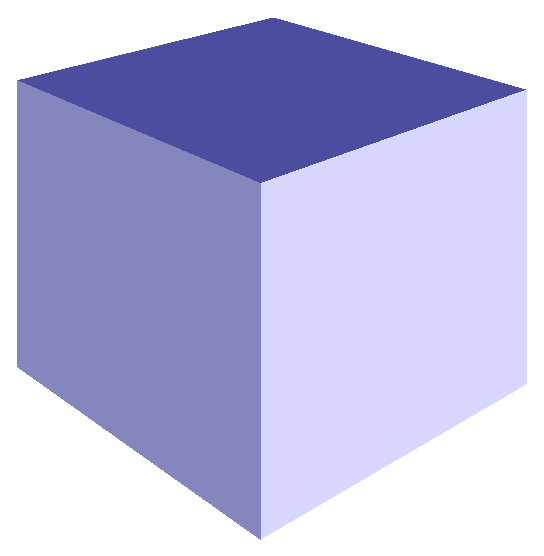
\includegraphics[width=0.1\textwidth]{cube.eps}\hspace{0.5cm}
    Cubic lattices
    \begin{itemize}
        \vspace{0.25cm}
        \item \ \pause Global synchronization does not occur for dimensions 2 or less
        \vspace{0.25cm}
        \item \ \pause Coupling function depends on the vertex position $i$:\\
            $\Gamma_i = \exp \left( a\frac{k_i^{x_i+1} - k_i^{x_i}}{2d} \right)$
        \vspace{0.25cm}
        \item \ \pause Evidence that the infinite period transition is absent for finite dimensional lattices with short range interactions.
        \vspace{0.25cm}
        \item \ \pause Behavior of the system for large couplings is similar to nucleation processes
    \end{itemize}
\end{frame}

\begin{frame}
    \centering
    Cluster growth at high coupling in a square lattice\\
    \vspace{0.8cm}
    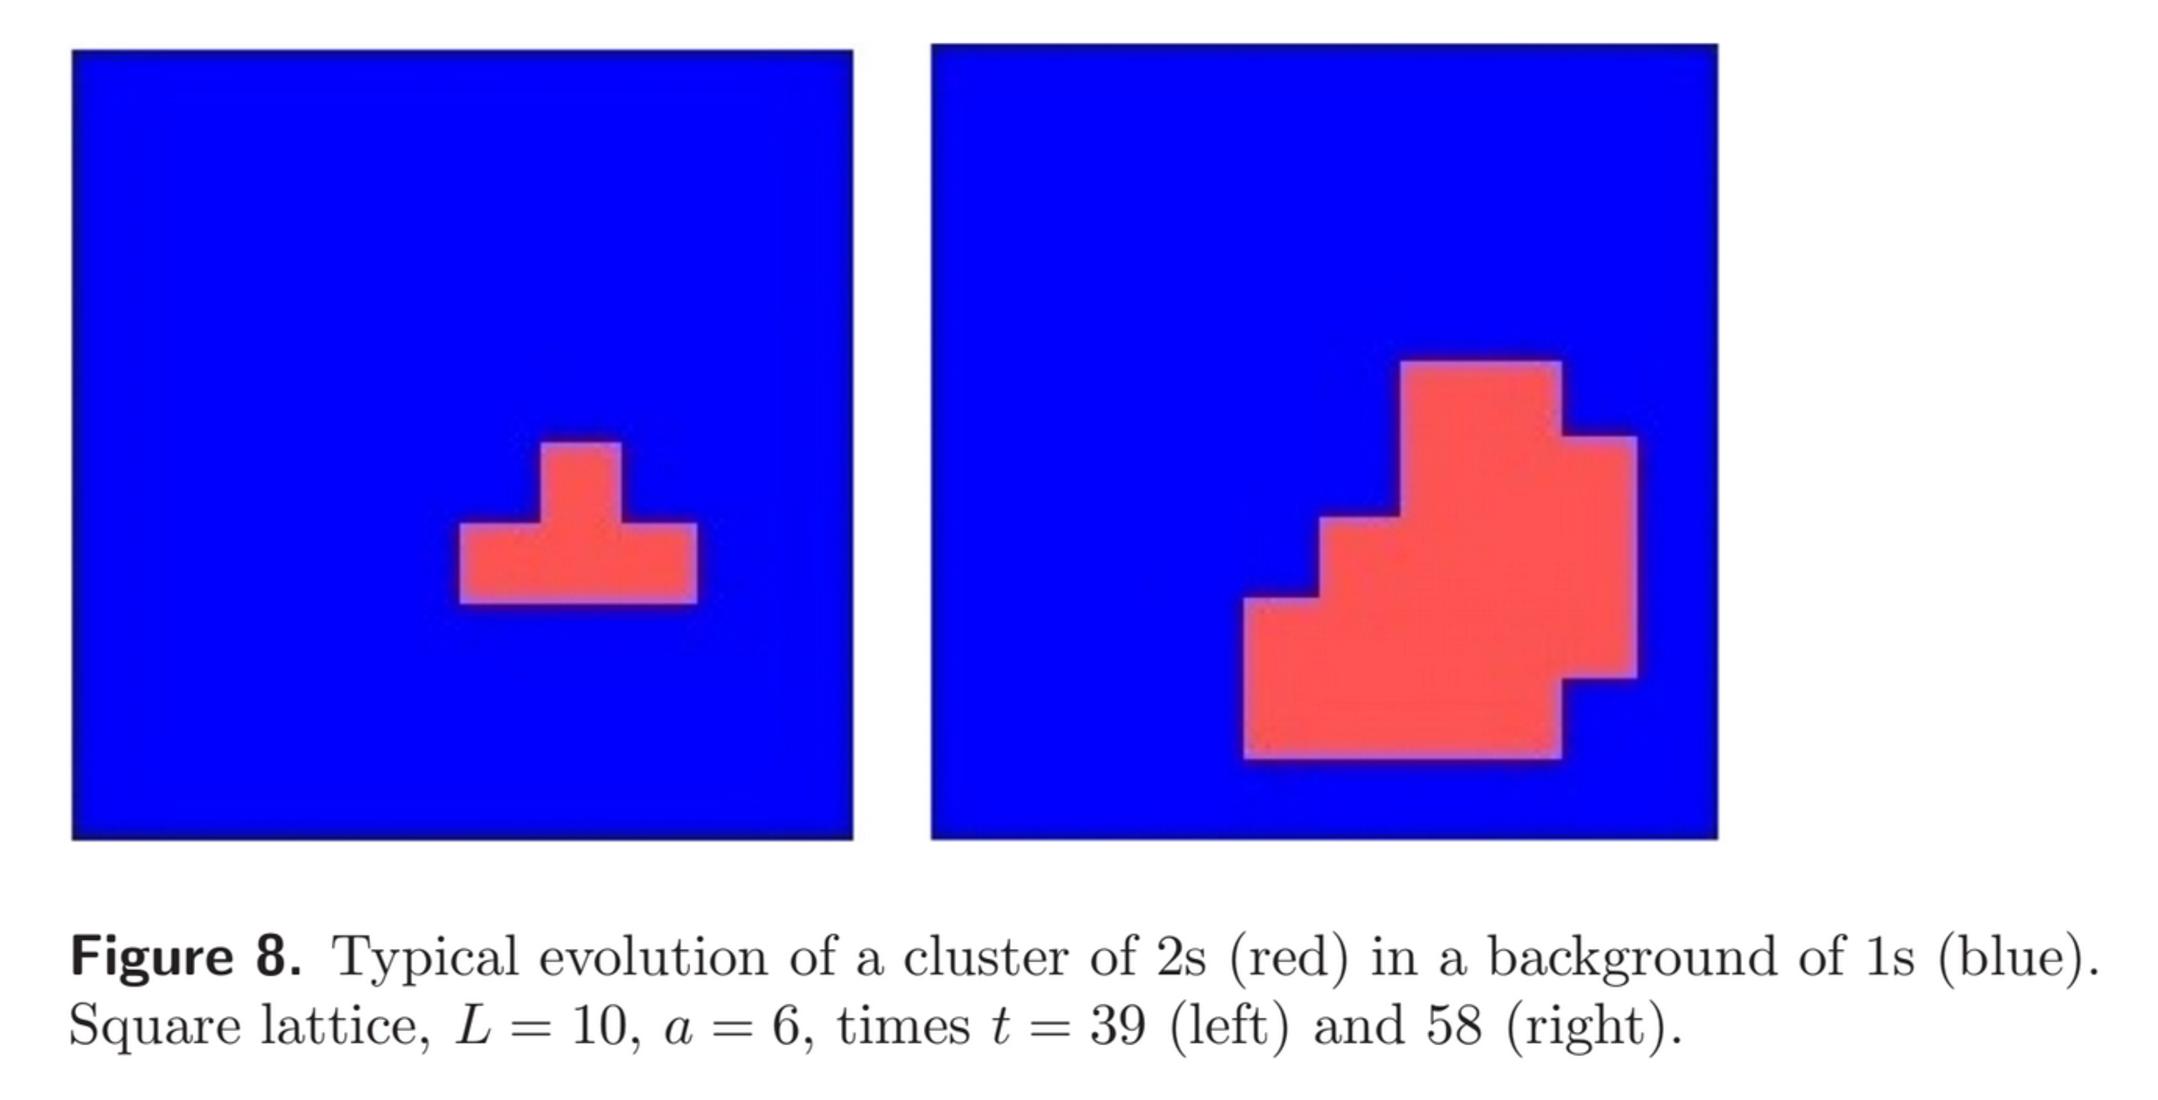
\includegraphics[height=0.6\textheight]{nucleation.eps}\\
    Vladimir R V Assis et al J. Stat. Mech. (2011) P09023
\end{frame}

\begin{frame}
    \centering
    Escape time from homogeneous initial condition\\
    \vspace{0.8cm}
    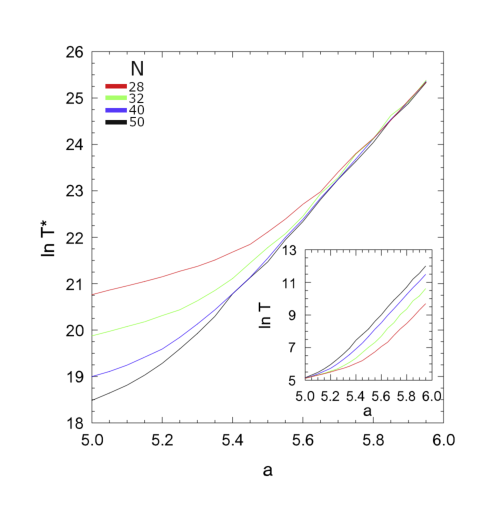
\includegraphics[height=0.75\textheight]{escapetime.eps}\\
    Vladimir R V Assis et al J. Stat. Mech. (2011) P09023
\end{frame}

\begin{frame}
    \begin{columns}
        \begin{column}{.5\textwidth}
            \adjincludegraphics[width=\textwidth, valign=t]{ring.eps}\\
            \vspace{0.1cm}
            N=12, K=2
        \end{column}
        \begin{column}{.5\textwidth}
            \textbf{Ring lattices}
            \begin{itemize}
                \vspace{0.25cm}
                \item \ \pause $N$ vertices connected to $2K$ neighbors each
                \vspace{0.25cm}
                \item \ \pause $\alpha = K/N$
                \vspace{0.25cm}
                \item \ \pause $0 \leq \alpha \leq 1/2$: 1D ring to all-to-all graph
                \vspace{0.25cm}
                \item \ \pause Range from local to global
            \end{itemize}
        \end{column}
    \end{columns}
\end{frame}

\begin{frame}
    \begin{columns}
        \begin{column}{.5\textwidth}
            \adjincludegraphics[height=0.4\textheight, valign=t]{ring.eps}\\
            \vspace{0.1cm}
            \adjincludegraphics[height=0.4\textheight, valign=t]{rewiredring.eps}\\
            N=12, K=2, p=0.1
        \end{column}
        \begin{column}{.5\textwidth}
            The \textbf{Watts-Strogatz} for \textbf{Small World} graphs
            \begin{itemize}
                \vspace{0.25cm}
                \item \ \pause We start from a ring graph
                \vspace{0.25cm}
                \item \ \pause Loop through each edge once, and with probability $p$ rewire its clock-wise vertex to another randomly selected vertex
                \vspace{0.25cm}
                \item \ \pause Forbid self-connections, overlapping connections or disconnected graphs
                \vspace{0.25cm}
                \item \ \pause $p$ and $K$ become parameters that alter the graphs connectivity
            \end{itemize}
        \end{column}
    \end{columns}
\end{frame}

\begin{frame}
    Small-world graphs are characterized by the \textbf{Clustering Coefficient $C$} and the \textbf{Average Path Length $L$} between nodes.\\
    \begin{itemize}
        \vspace{0.25cm}
        \item \textbf{Clustering Coefficient}: let $K_i$ be the number of neighbors of vertex $i$. Then, there are at most $K_i(K_i-1)/2$ connections between them. If we divide the number of \emph{actual} connections between them by the \emph{maximum} number of connections, we get a number $C_i$. $C$ is given by the average $C_i$ over the entire graph
        \vspace{0.25cm}
        \item \textbf{Average Path Length}: Given two vertices $i$ and $j$, let $L_i$ be the minimum number of edges traversed to get from $i$ to $j$. Then $L$ is given by the average $L_i$ over the entire graph
    \end{itemize}
\end{frame}

\begin{frame}
    \centering
    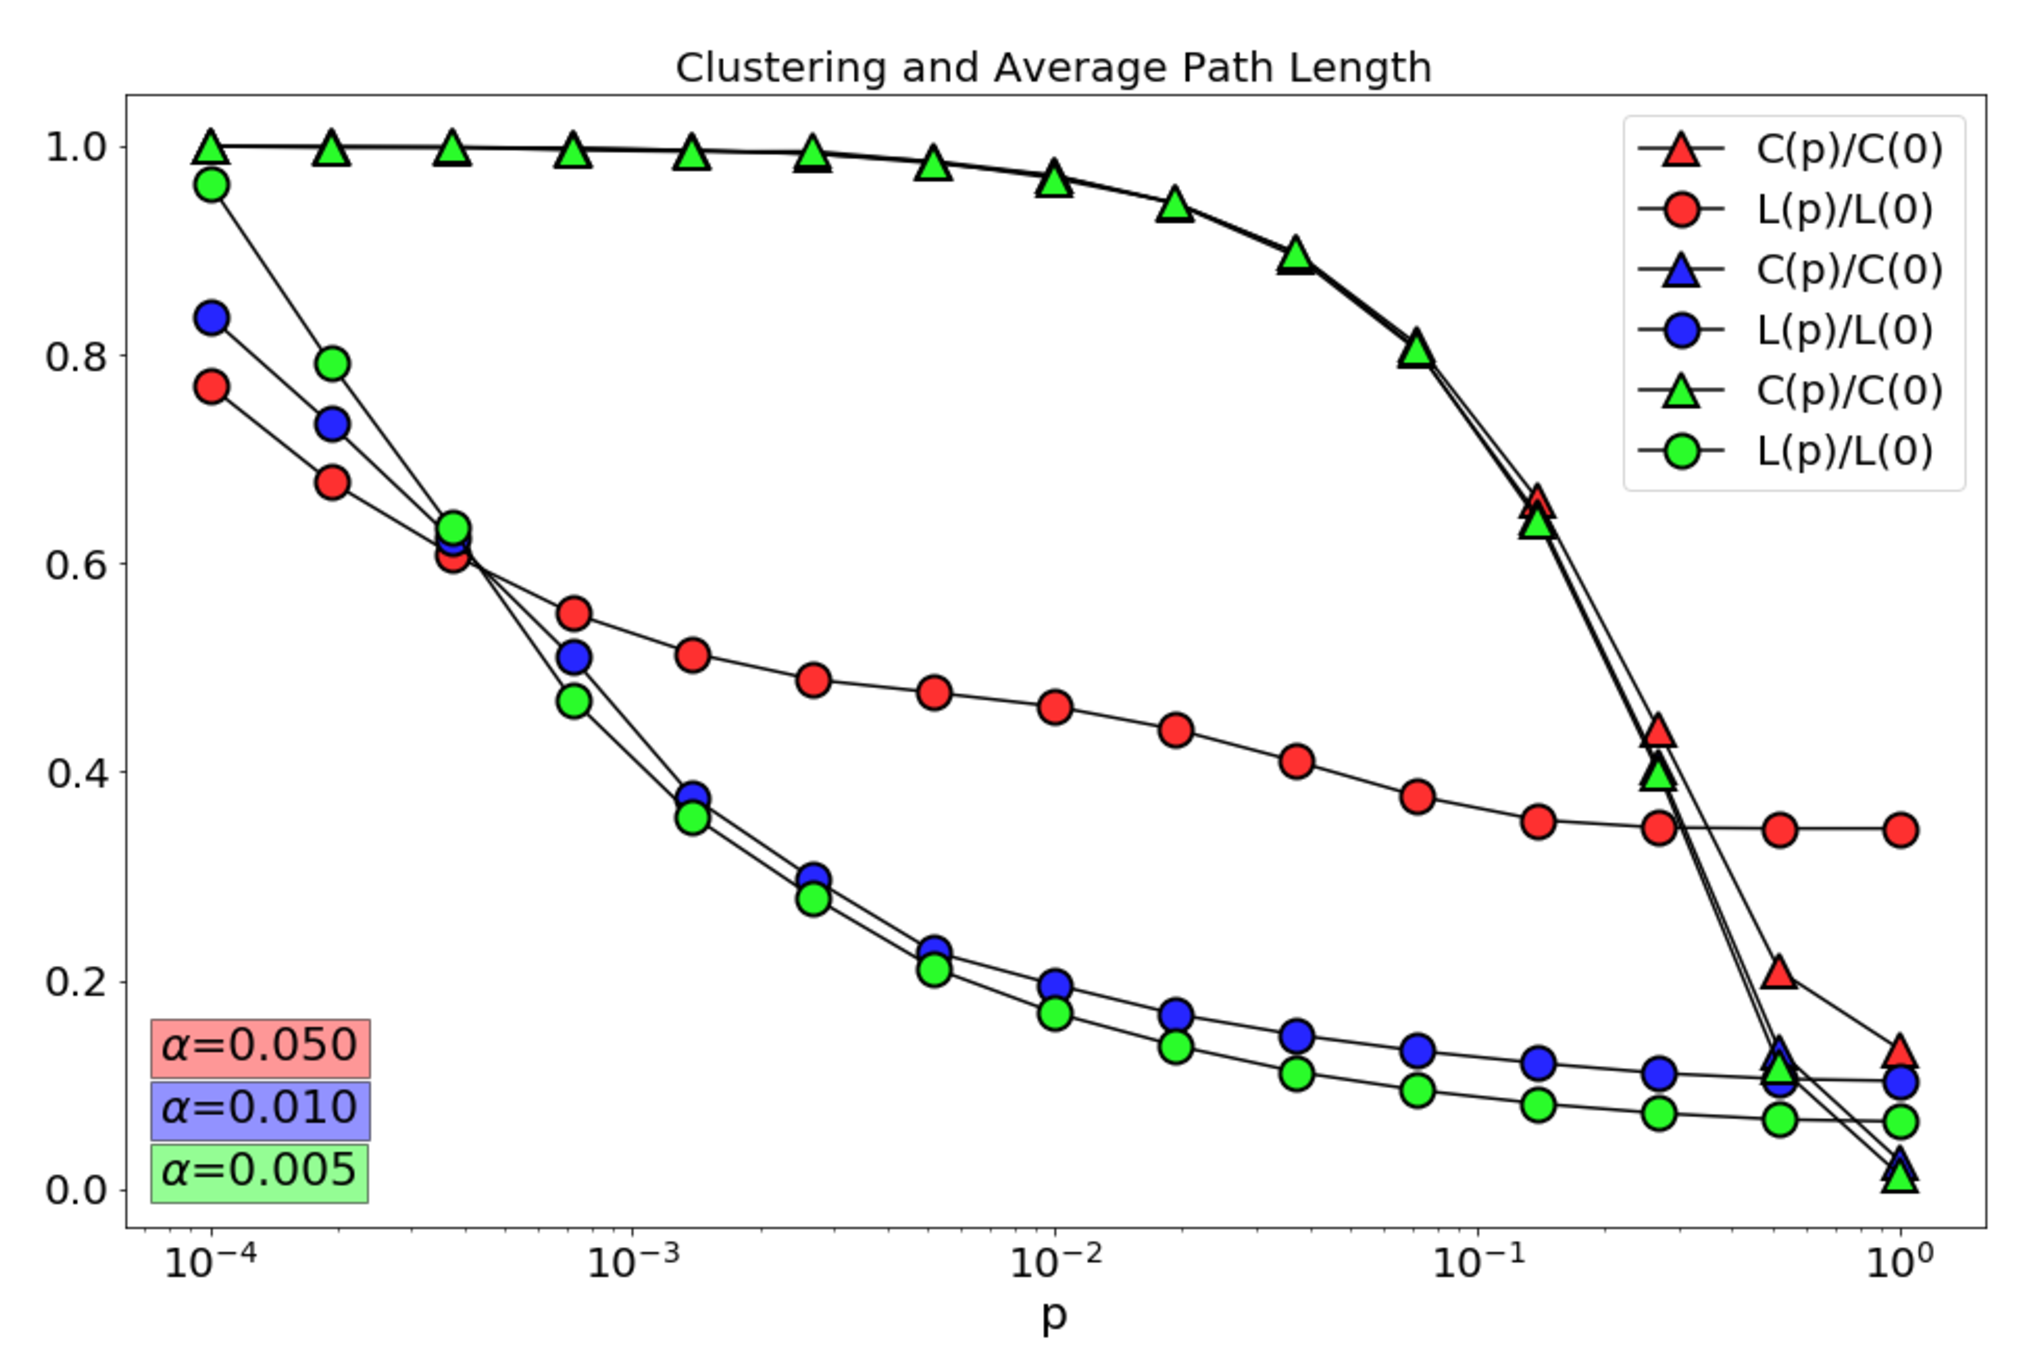
\includegraphics[height=0.85\textheight]{small-world.eps}
\end{frame}

\begin{frame}
    \begin{columns}
        \begin{column}{0.4\textwidth}
            \adjincludegraphics[height=0.35\textheight, valign=t]{ring-1D.eps}\\
            N=12, K=1
            \adjincludegraphics[height=0.35\textheight, valign=t]{ring-Complete.eps}\\
            N=5, K=2
        \end{column}
        \begin{column}{0.6\textwidth}
            How does the coupled oscillator dynamics evolve in different ring lattices?\\
            \vspace{0.25cm}
            \begin{itemize}
                \vspace{0.25cm}
                \item \ \pause For $K/N \approx 0$ we know there is no global synchrony (1D cubic lattice with periodic boundary)
                \vspace{0.25cm}
                \item \ \pause For $K/N\rightarrow 0.5$ there must exist two transitions
                \vspace{0.25cm}
                \item \ \pause We investigate the behavior of the system through event driven simulations
            \end{itemize}
        \end{column}
    \end{columns}
\end{frame}

\begin{frame}
    \centering
    Population evolution on a ring lattice with N=10000 K=1280\\
    \vspace{0.8cm}
    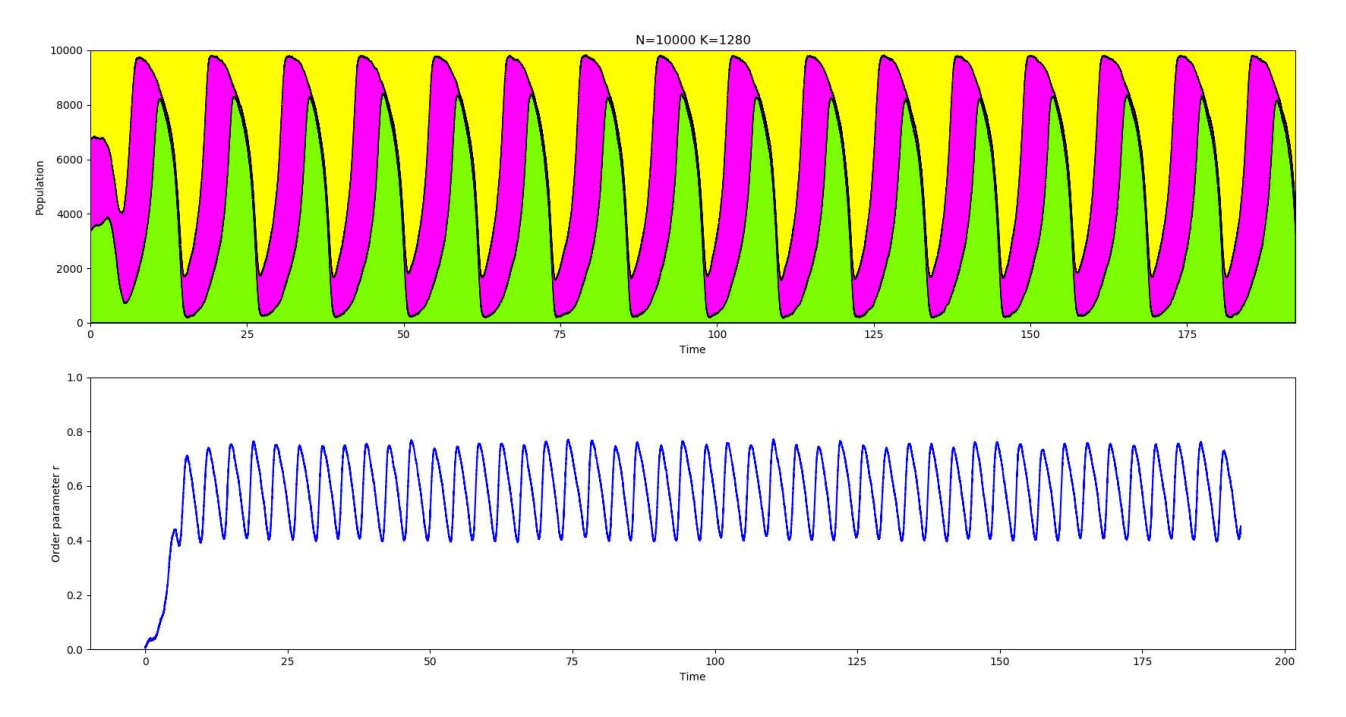
\includegraphics[width=\textwidth]{pop-evolution-stacked-K_1280.eps}
\end{frame}

\begin{frame}
    \centering
    Population evolution on a ring lattice with N=10000 K=160\\
    \vspace{0.8cm}
    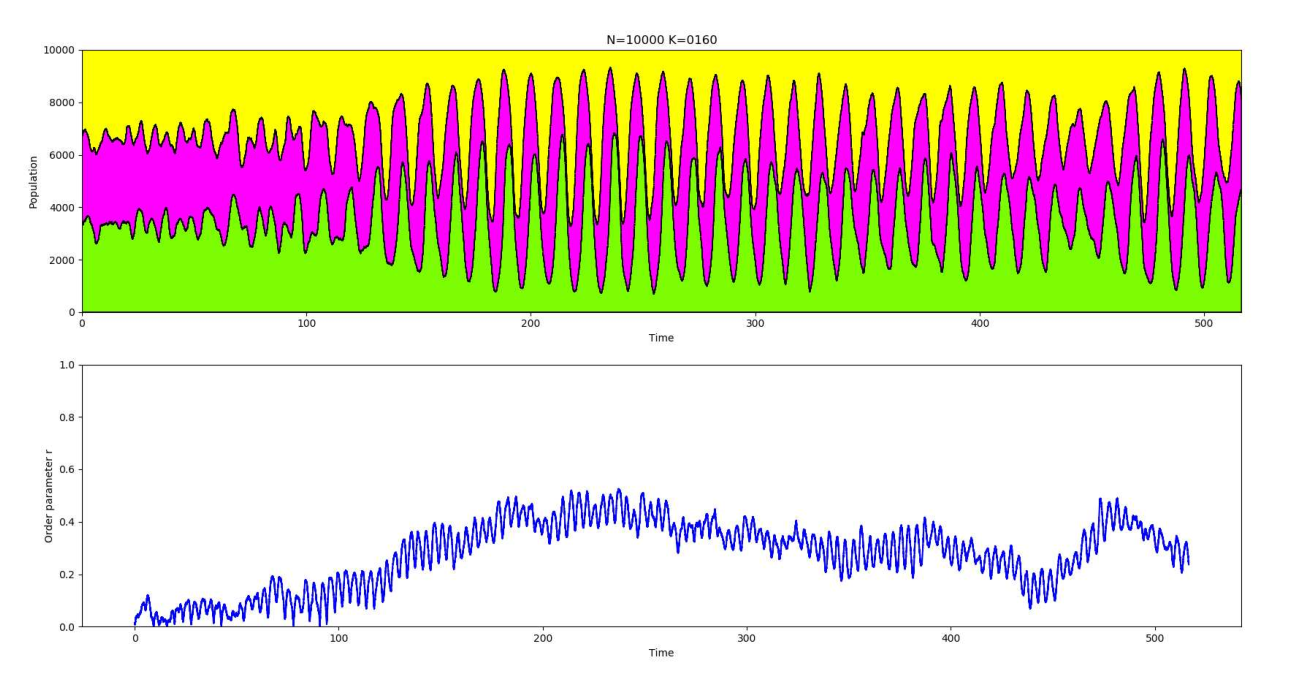
\includegraphics[width=\textwidth]{pop-evolution-stacked-K_160.eps}
\end{frame}

\begin{frame}
    \centering
    Population evolution on a ring lattice with N=10000 K=80\\
    \vspace{0.8cm}
    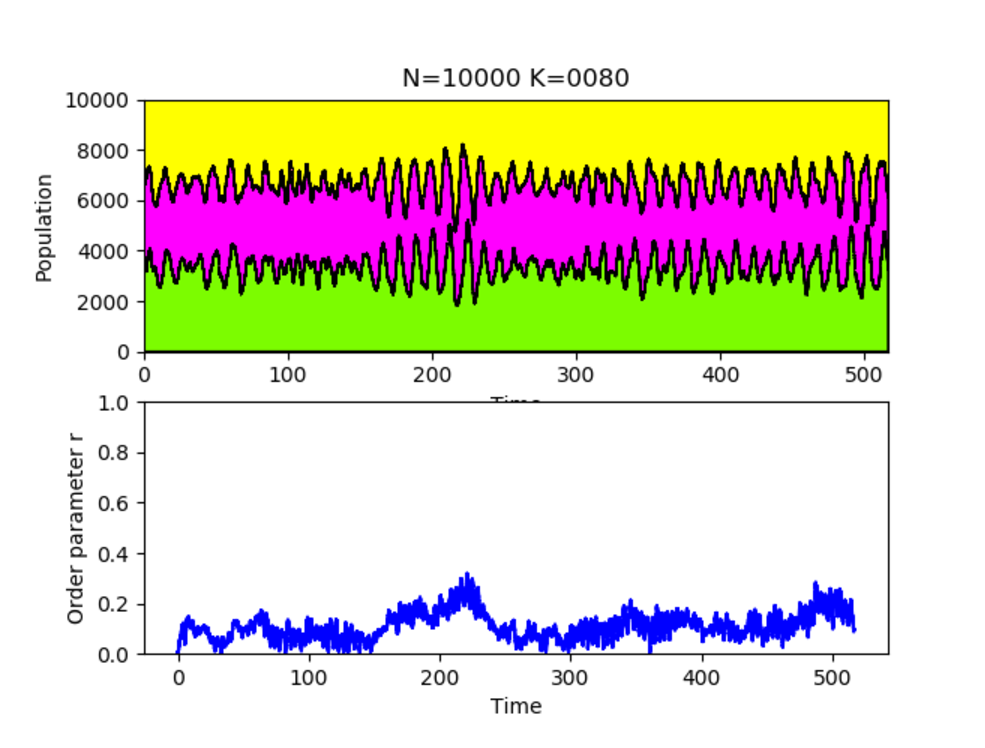
\includegraphics[width=0.8\textwidth]{pop-evolution-stacked-K_80.eps}
\end{frame}

\begin{frame}
    \centering
    Fixed system size, increasing $K$ (or $\alpha$)\\
    \vspace{0.25cm}
    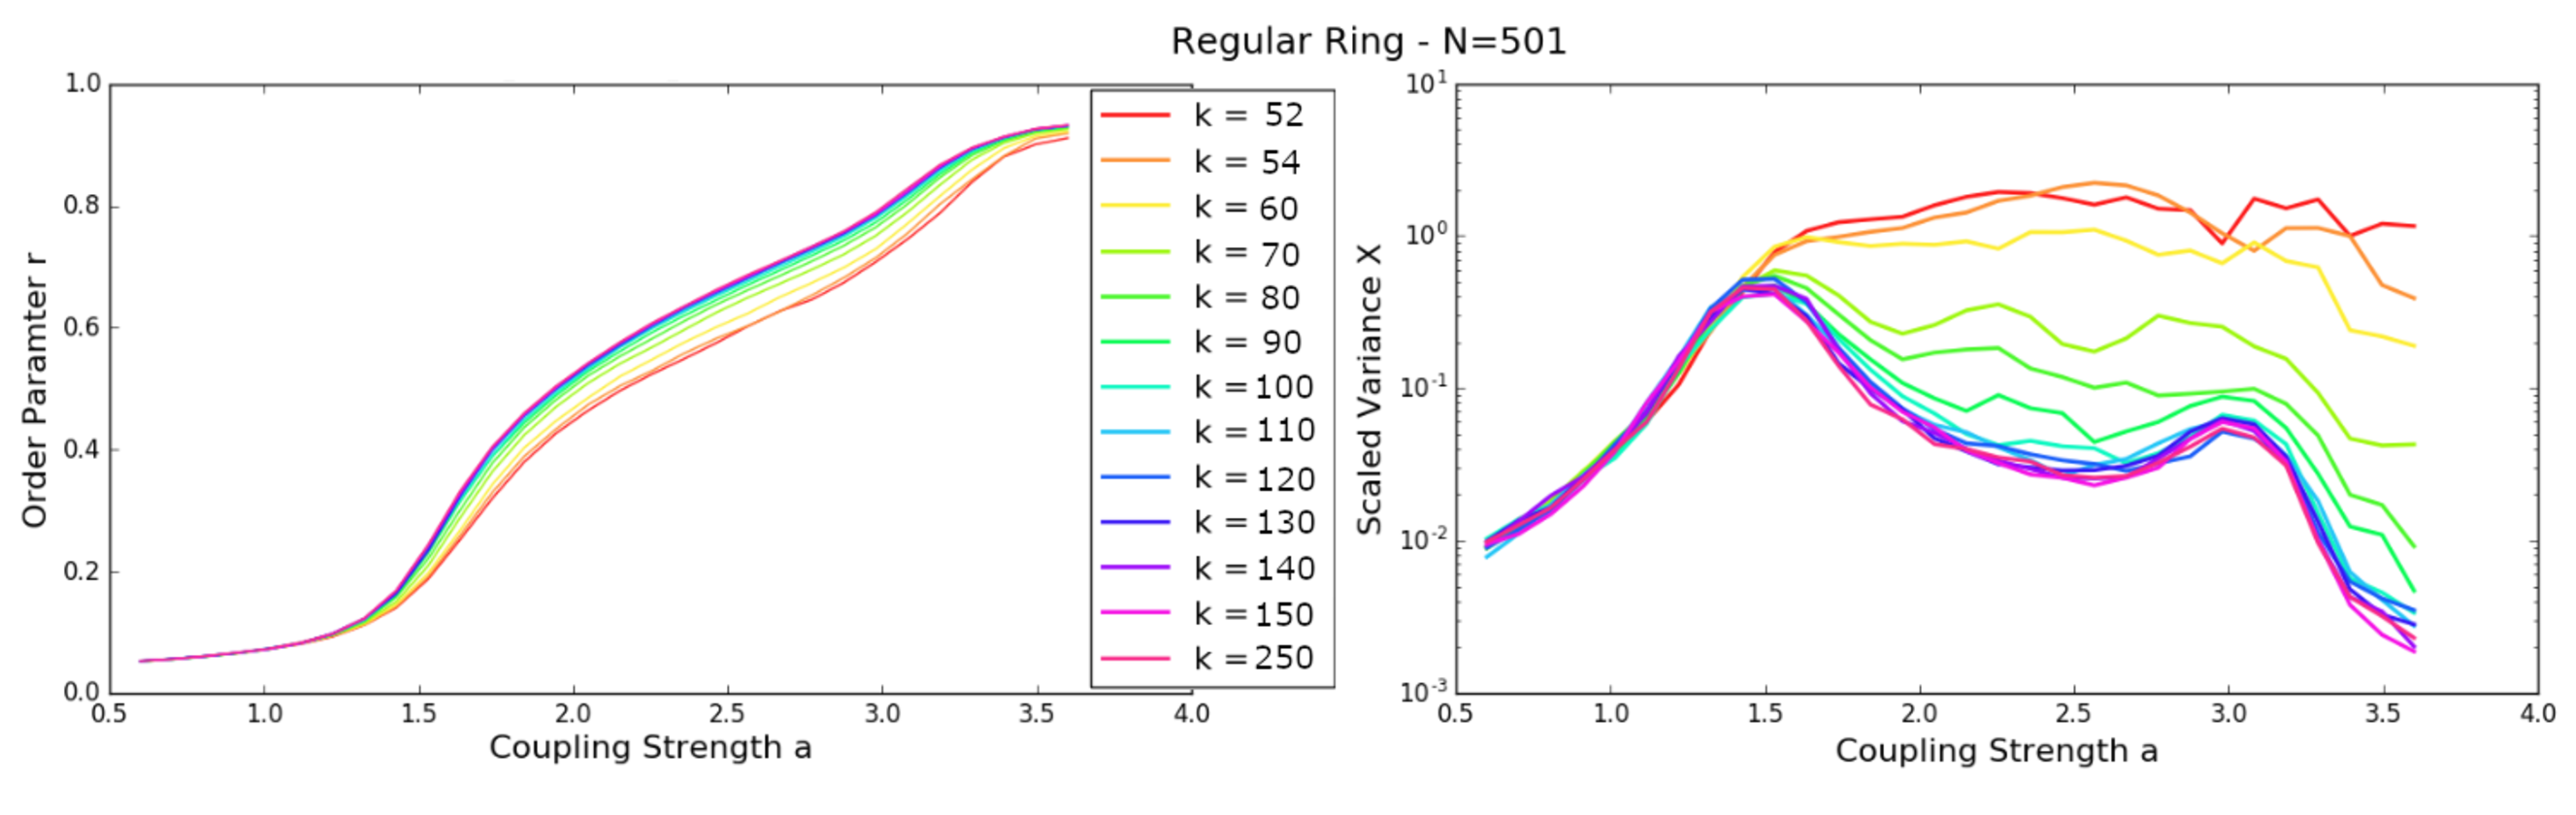
\includegraphics[width=\textwidth]{ringOP.eps}
\end{frame}

\begin{frame}
    \centering
    Behavior for fixed $\alpha=0.1$ and increasing system size $N$\\
    \vspace{0.25cm}
    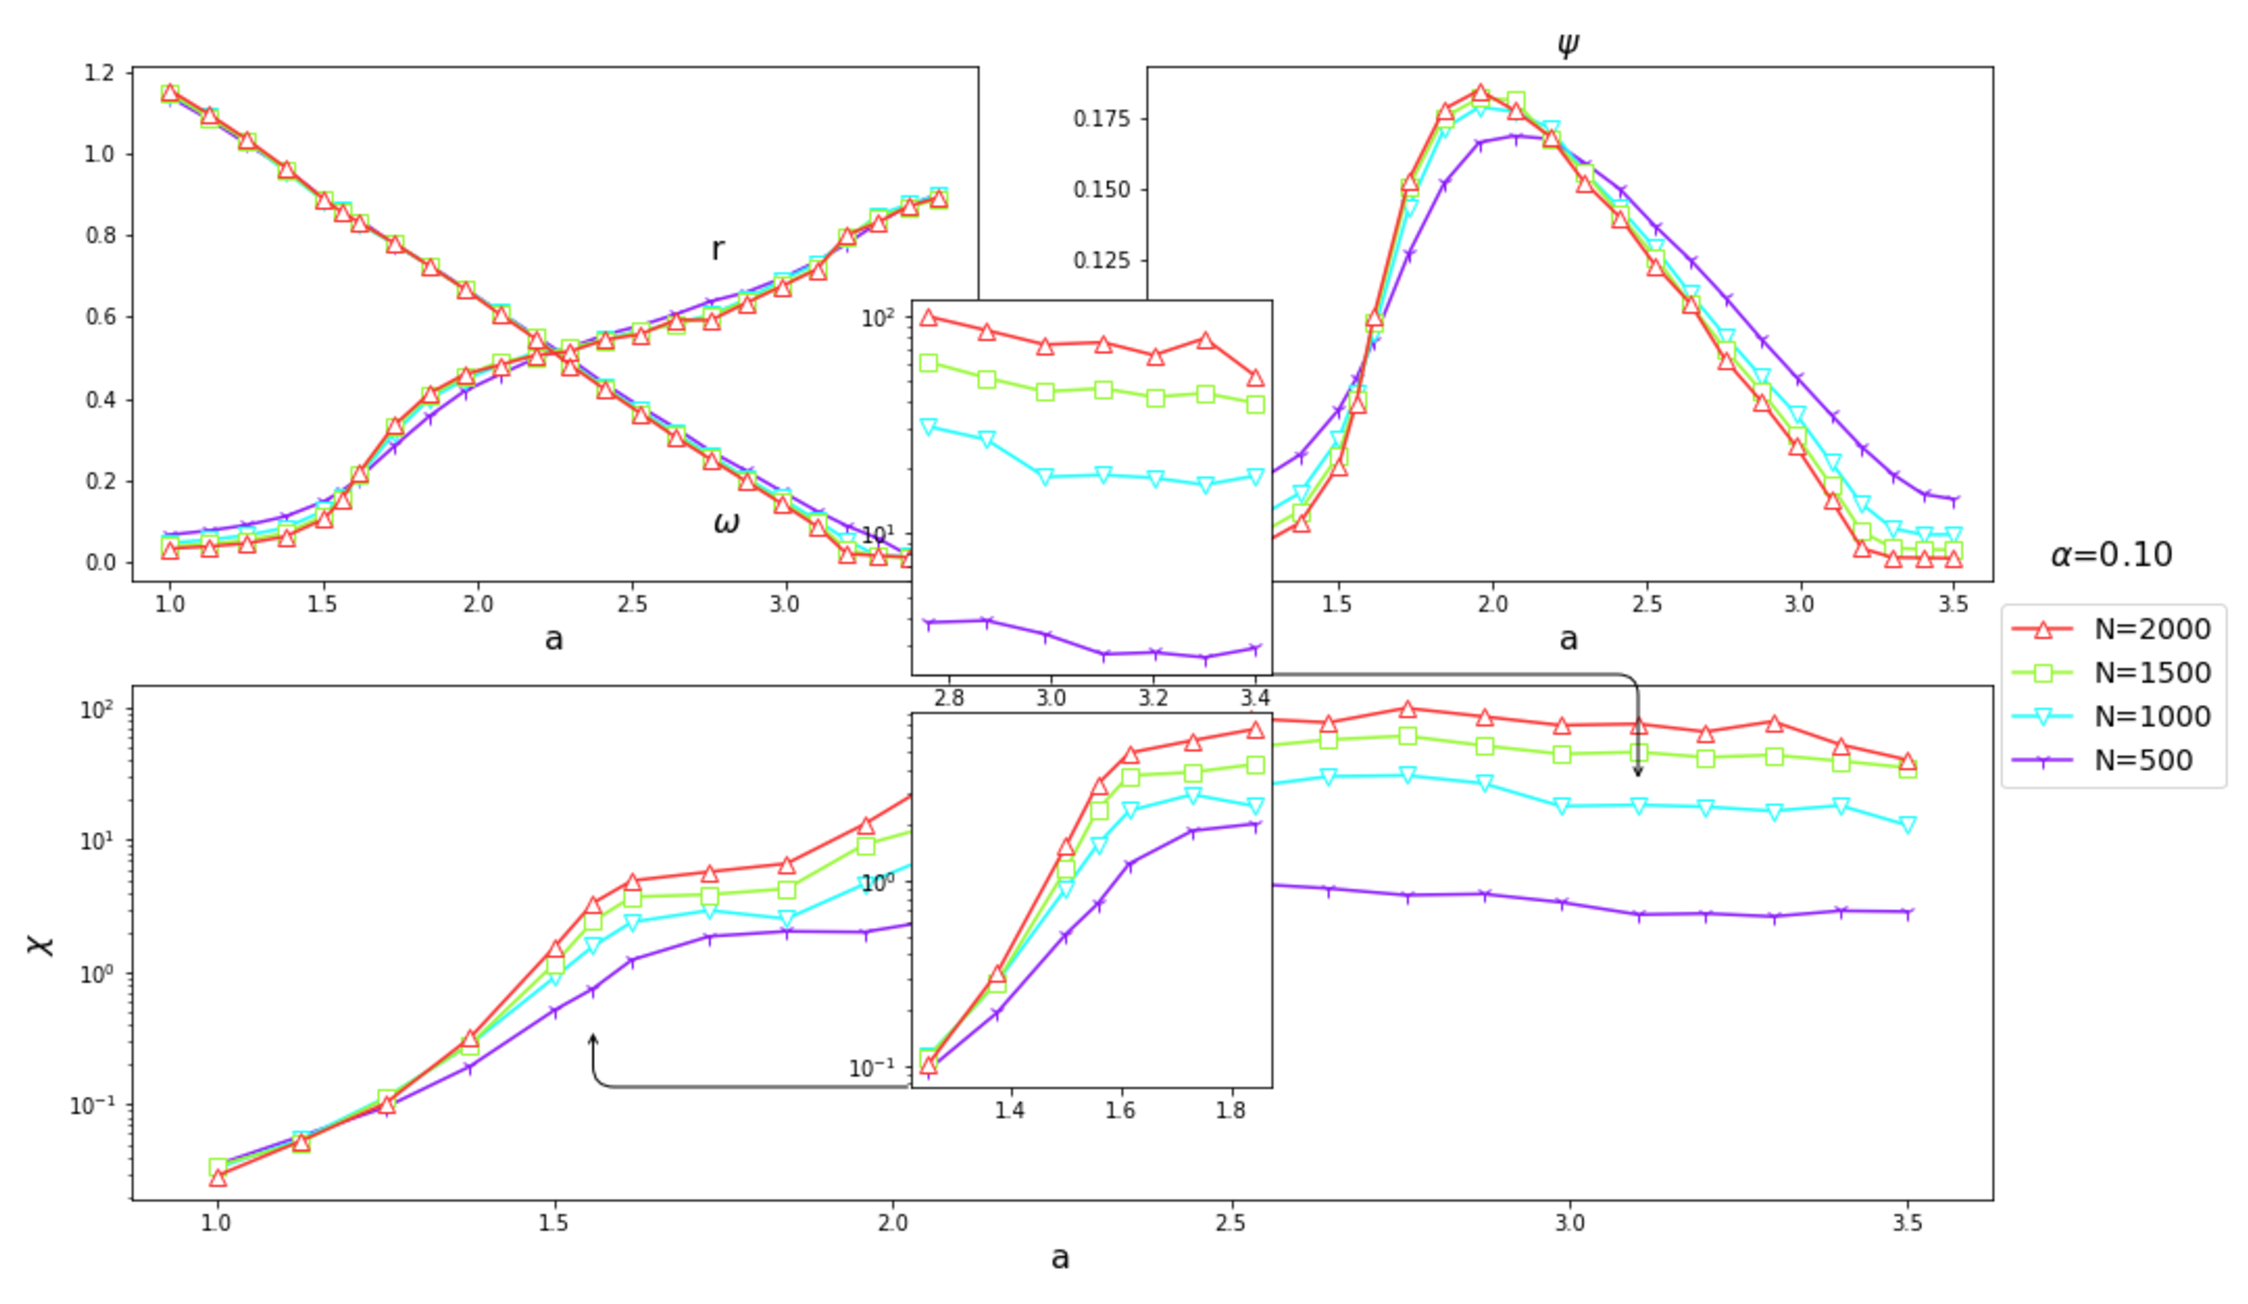
\includegraphics[width=0.8\textwidth]{increasingN-alpha10.eps}
\end{frame}

\begin{frame}
    \centering
    Behavior for fixed $\alpha=0.34$ and increasing system size $N$\\
    \vspace{0.25cm}
    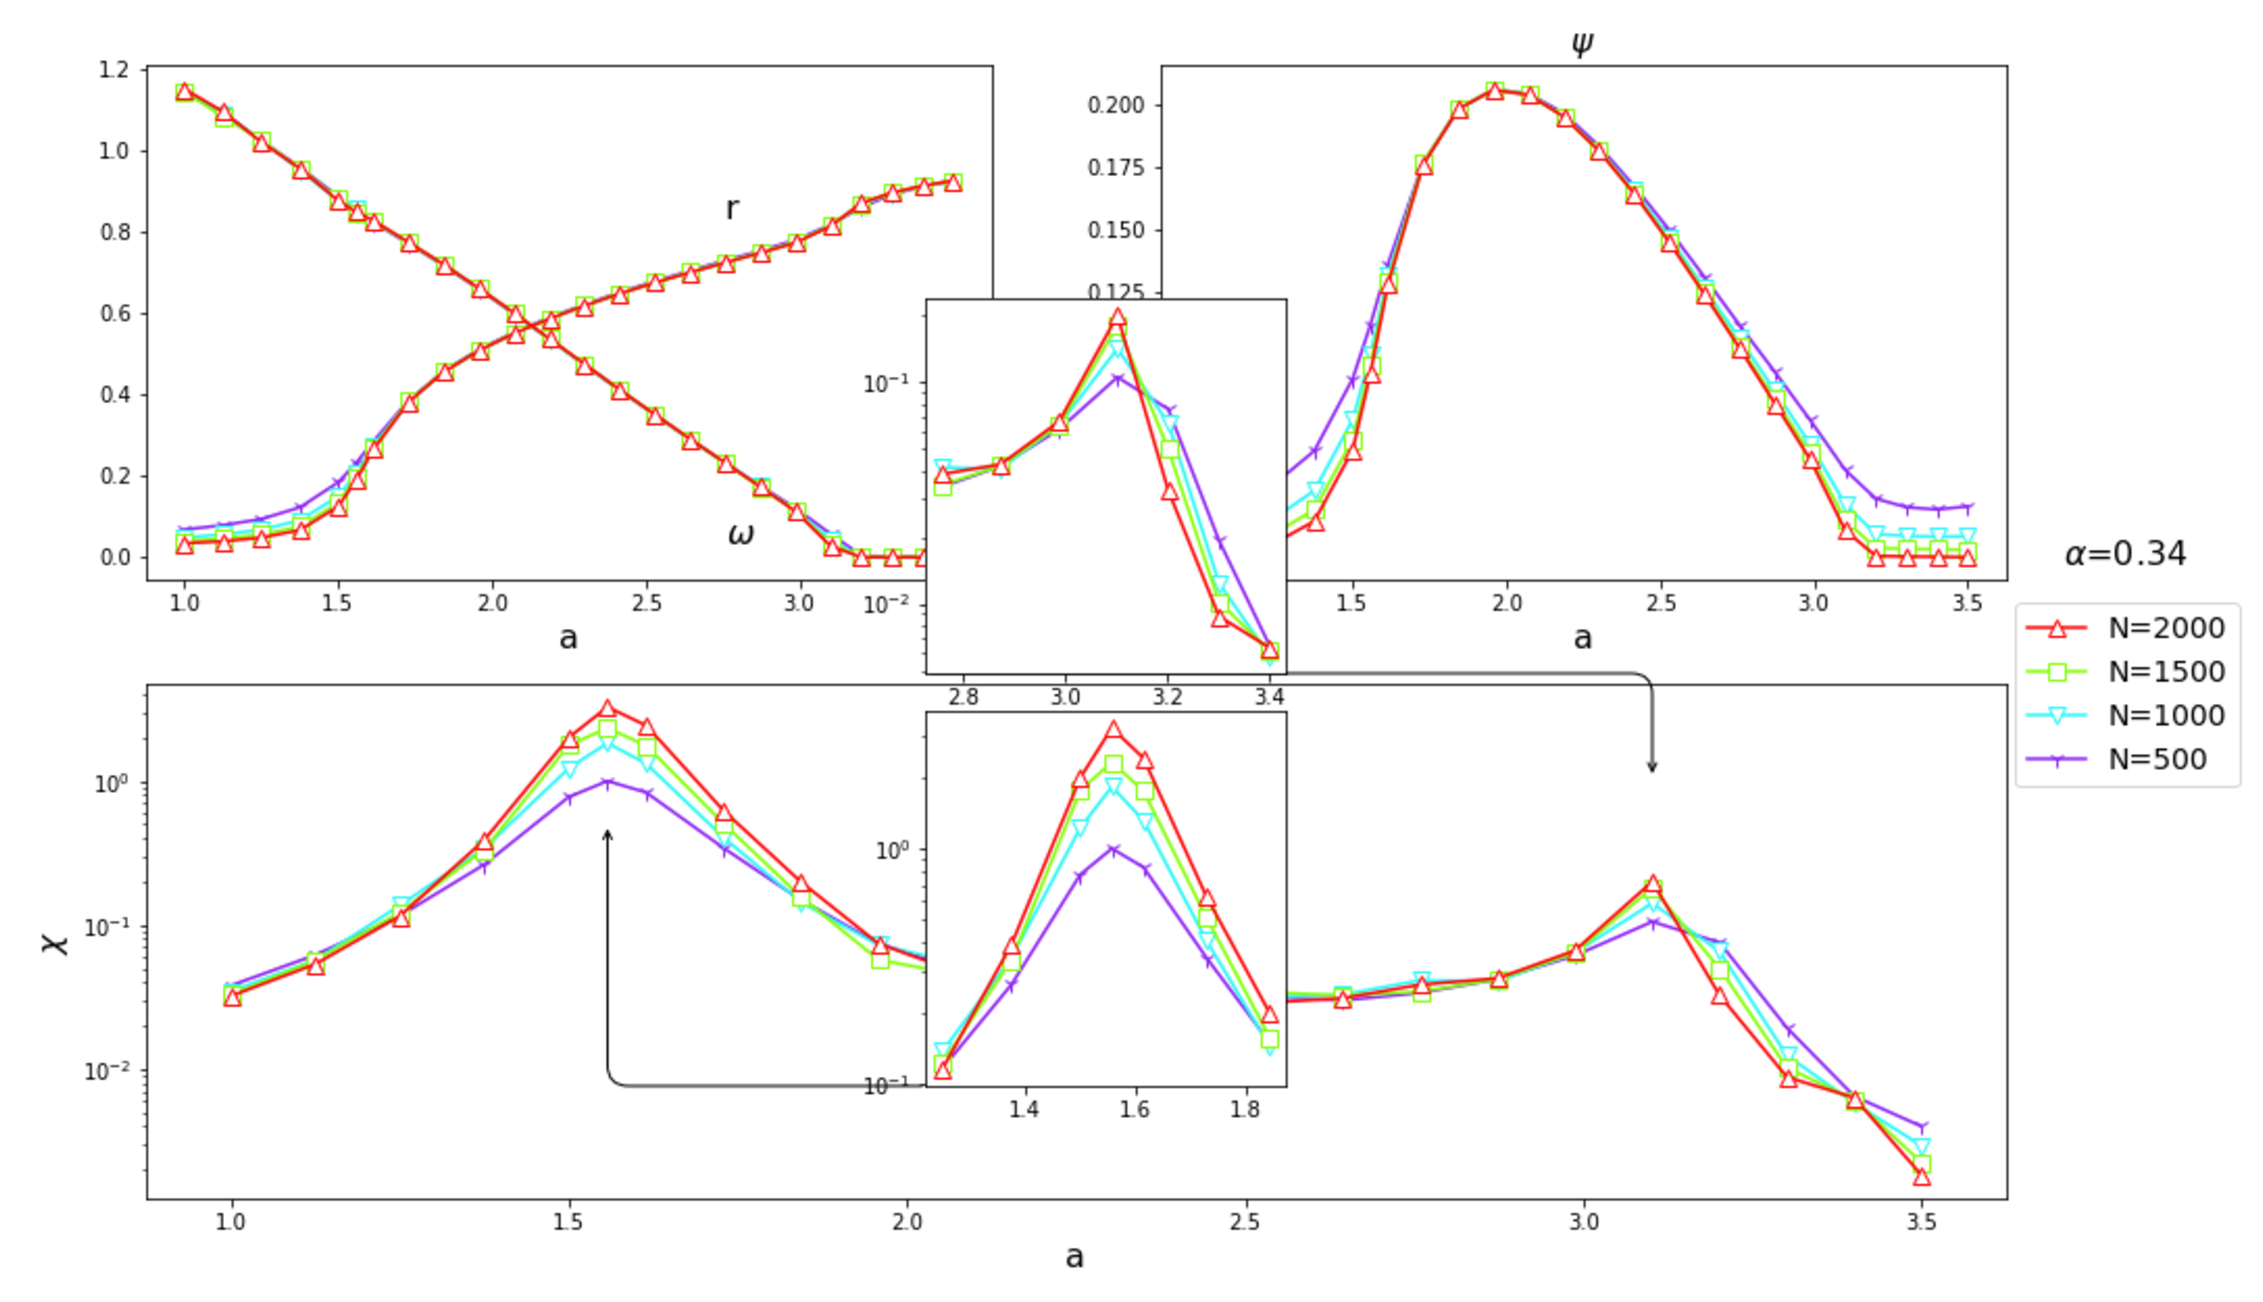
\includegraphics[width=0.8\textwidth]{increasingN-alpha34.eps}
\end{frame}

\begin{frame}
    \centering
    Fixed $N$ and $K$, increasing $p$\\
    \vspace{0.25cm}
    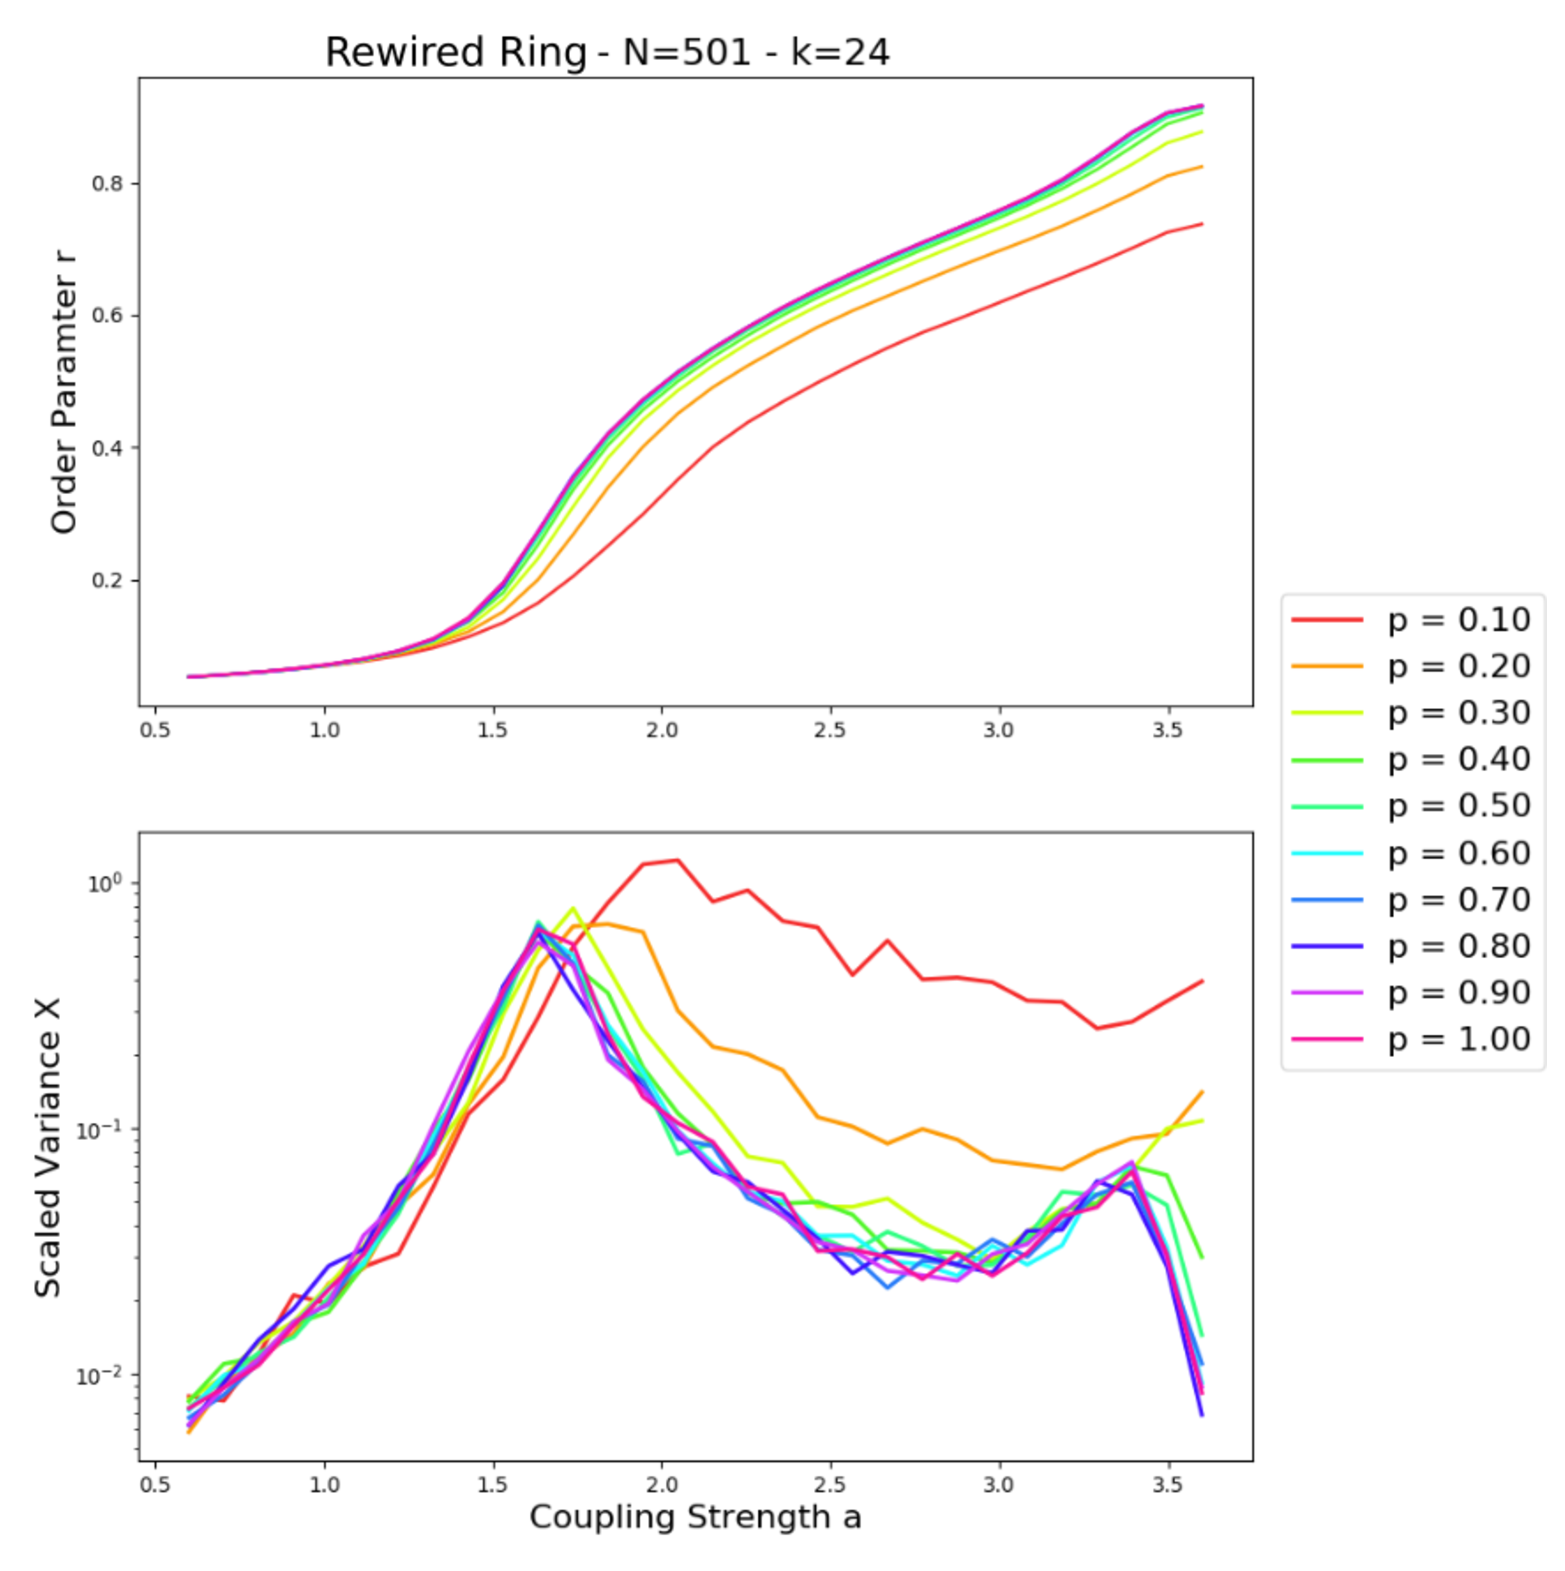
\includegraphics[height=0.8\textheight]{rvsavsp.eps}
\end{frame}

\begin{frame}{Conclusions and Discussion}
    \begin{itemize}
        \item \ \pause The phase transitions seem to exist on ring graphs for intermediate values of $\alpha$. Even for $\alpha=0.1$ the behavior of $\psi$ and $\omega$ indicate a transition, though $\chi$ behaves differently.
        \vspace{0.1cm}
        \item \ \pause Increasing the rewiring probability has similar effects to increasing connectivity. This is expected according to Duncan J. Watts and Steven H. Strogatz.\\
            \hfill -- "Collective dynamics of ‘small-world’networks." nature (1998)
        \vspace{0.1cm}
        \item \ \pause Although $p>0$ facilitates synchronicity, it is not necessary for the onset of global synchronicity even for low values of $\alpha$.
        \vspace{0.1cm}
    \item \ \pause As of yet, it is unclear whether $p>0$ is required for the transition to infinite period and the breaking of the $C_3$ rotational symmetry this system presents.
    \end{itemize}
\end{frame}

\begin{frame}{Some broad strokes about the future\dots}
    \begin{itemize}
        \item \ \pause I am interested in the process of learning
        \item \ \pause Currently there are models that simulate associative memories through the recovery of spatial patterns, such as the Hopfield model for associative memory and other ``Ising-like'' models
        \item \ \pause The discrete oscillators model has the potential to perform similar tasks but with the addition of temporal patterns (e.g. multiple stable frequencies)
        \item \ \pause No idea how to train such a model (many studies of associative memories do not concern about the learning phase though)
    \end{itemize}
\end{frame}

\begin{frame}
  \frametitle{Questions}
\end{frame}

\end{document}

